% Latex Template
%
% Fall 2015
%
% Created by: Andy Sayler
% Modified by: Taylor Andrews

\documentclass[11pt,twocolumn,letterpaper]{article}

% System Packages
\usepackage{epsfig}
\usepackage{float}
\usepackage{caption}
\usepackage{subcaption}
\usepackage{tabu}
\usepackage{color}
\usepackage{hyperref}
\usepackage{url}

% Local Packages
% None

% Package Options
\hypersetup{
    colorlinks,
    citecolor=black,
    filecolor=black,
    linkcolor=black,
    urlcolor=black
}

% Macros
\newenvironment{packed_enum}{
\begin{enumerate}
  \setlength{\itemsep}{1pt}
  \setlength{\parskip}{0pt}
  \setlength{\parsep}{0pt}
}{\end{enumerate}}

\newenvironment{packed_item}{
\begin{itemize}
  \setlength{\itemsep}{1pt}
  \setlength{\parskip}{0pt}
  \setlength{\parsep}{0pt}
}{\end{itemize}}

\newenvironment{packed_desc}{
\begin{description}
  \setlength{\itemsep}{1pt}
  \setlength{\parskip}{0pt}
  \setlength{\parsep}{0pt}
}{\end{description}}


% Other Options
\clubpenalty = 10000
\widowpenalty = 10000

% Variable
\newcommand{\appname}{Custos FuseBox }
\newcommand{\appnameWOspace}{Custos FuseBox}

% Start
\begin{document}

\title{\appname}

\author{Taylor Andrews}

\maketitle

\begin{abstract}
Security in the digital age is an ever evolving problem.
Services are doing their very best to protect sensitive data. 
However, in the face of social engineering attacks and other more technical
exploits, it can be on the user to go the extra step to make sure
their data is safe. Safety, however, should not come at the cost of
sharing data between trusted people and devices. Take Dropbox for
example CITATION?. It supports many sharing features, so users can't just
encrypt and decrypt their files on a single computer. A more robust,
and shareable, way to encrypt files is needed. 
\par \appname aims to be a solution to this problem by providing a
transparent layer of security between the end user and Dropbox. Files
that pass through \appname are encrypted when uploaded to Dropbox. 
Thus, using the client guarantees that data is protected even if 
Dropbox is compromised. This fulfills the need for safety. The need
for shareability
is accomplished using Custos, a ``Secret Storage as a Service''
(SSaaS) platform CITATION?. Custos allows for key sharing amongst
people and computers. This paper will lay out
the design and implementation of \appnameWOspace, as well as 
future goals for the project.    
\end{abstract}

\section{Introduction}
\label{sec:intro}
Unsecured data is a gamble, a risk. No one wants to think that
they could be the target of an attack. The idea of keeping things safe
is nothing complicated. However, to the layman, the intricacies of
actually protecting data are somewhat out of reach. This problem
becomes compounded when a single person wants to safely share data
with trusted partners. Fortunately, part of the solution already exits.
Custos, a SSaaS, provides a flexible means of storing and
retrieving secrets CITATION?. Leveraging Custos allows \appname to 
encrypt and authenticate in conjunction with cloud based services.      
\par 
Accessible security is the aim of \appnameWOspace. This starts with
creating a client that's easy to understand. 
\par
\appname is the product of many different libraries. 

\subsection{Goals}
\label{sec:goals}
\appname was created to be a simple and transparent security
measure. Easy to setup, easy to use.
\par {\bf Transparency:} Dropbox is a very convenient application to
use. Put files in, get files out. The existing desktop application
allows for seamlessly uploading and downloading files CITATION?. The end user
gets to take advantage of all the nice features of Dropbox at little
to no effort on their end. \appname is built to keep this same 
seamless feel while preserving the features of Dropbox. meanwhile behind the
scenes encryption, decryption, and authentication work together to
secure the data.     
\par {\bf Simplicity:} 

\section{Design}
\label{sec:design}

Design Section

\section{Implementation}
\label{sec:implementation}

This is another section.

%\section{Evaluation}
%\label{sec:eval}

\section{Conclusion}
\label{sec:conclusion}

Where do we go from here?

\section{Examples}
\label{sec:ex}

\noindent
This is a citation~\cite{exampleref1}.

% The tilde (~) in the previous sentence is optional, and just helps
% to insure citations and references don't wind up on a new line
% separated from the text they're attached to.

% noindent can be used to prevent indentation on single-line paragraphs.

\begin{figure}[htb]
  \centering
  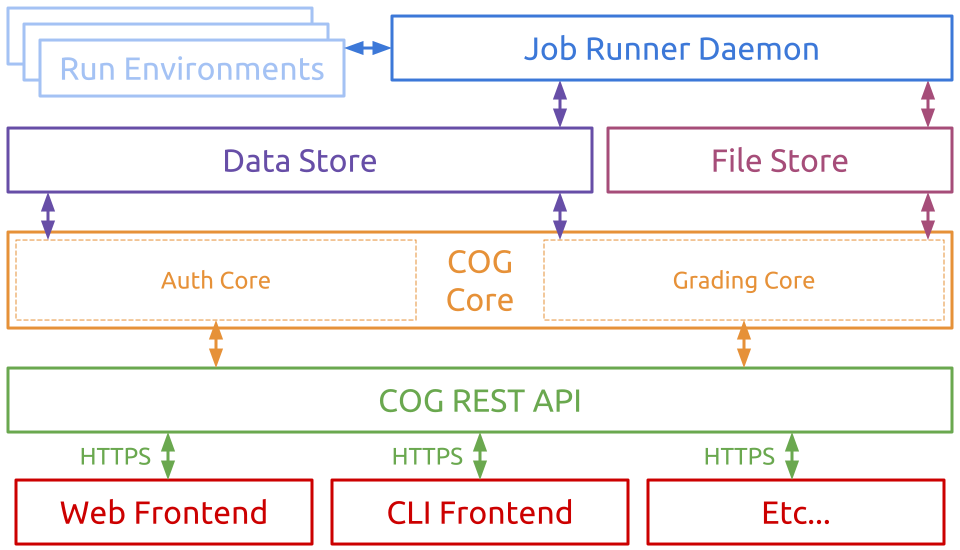
\includegraphics[width=\columnwidth]{./figs/pdf/examplefig1.pdf}
  \caption{Example Figure 1}
  \label{fig:example1}
\end{figure}

\noindent
Figure~\ref{fig:example1} is an example figure. The proceeding
sentence contains a reference to it.

\noindent
Sometimes you want thing in {\bf bold}.

\noindent
Or in {\em italics}.

\noindent
Or in \texttt{type-write font}.

\noindent
Sometime you need to do some math: $9/3=3$.

\noindent
Or ``a quote.''

\noindent
Or add a bullet list:

\begin{packed_item}
\item Item A
\item Item B
\item Item C
\end{packed_item}

\noindent
Or a numbered list:

\begin{packed_enum}
\item Item 1
\item Item 2
\item Item 3
\end{packed_enum}

\noindent
Or a definitions list:

\begin{packed_desc}
\item[Item I:] This is item 1 
\item[Item II:] This is item 2
\item[Item III:] This is item 3
\end{packed_desc}

% Note: The ``packed'' variants of the above items are my own and are
% defined in macros.tex. They are more tightly spaced versions of the
% standard LaTeX enumerate, itemize, and description environments.

\bibliographystyle{acm}
\bibliography{refs}

\end{document}
